Dans cette section on propose de valider l'implémentation des schémas
numériques décrits dans la section
(\ref{sec:fourier-discretisation}). Dans un premier temps, on
introduit une solution exacte du problème
(\ref{eq:stokes-u}),(\ref{eq:stokes-p}) qui satisfait les conditions
aux limites (\ref{eq:stokes-bc-1})-(\ref{eq:stokes-bc-3}). Dans un
deuxième temps, on analysera la convergence de l'erreur entre la
solution exacte et l'approximation $u_{h,K}$ telle que définie par
(\ref{eq:u-h-12}), (\ref{eq:u-h-3}).

\subsection{Une solution exacte polynomiale non triviale}
On pose $\Lambda = (-1, 1)^2$, on rappelle que $\Omega =
\Lambda\times(0,\thickness)$. On choisit dans cette partie
\ref{sec:fourier-validation} une viscosité scalaire unité,
c'est-à-dire que $\mu_{i,j} = 1\ \forall i,j$. On vérifie alors que les
fonctions $u_1, u_2, u_3:\Omega\to\mathbb R$ et $p:\Omega\to\mathbb R$
définies par:
\begin{align}
  &u_1(x_1, x_2, x_3) = u_2(x_1, x_2, x_3) = \parent{x_1^2 - 1}^2 %
  \parent{x_2^2 - 1}^2
  \parent{x_3^3 - \frac{3}{2}\thickness x_3^2 + \frac{1}{4}\thickness ^3},\label{eq:stokes-exact-sol-1}\\
  &u_3(x_1, x_2, x_3) = %
  \begin{aligned}[t]
    &\parent{-4x_1\parent{x_1^2 - 1} %
                                   \parent{x_2^2 - 1}^2 %
                              -4x_2\parent{x_2^2 - 1} %
                                   \parent{x_1^2 - 1}^2} \\
    &\cdot\parent{\frac{1}{4}x_3^4 - \frac{1}{2}\thickness x_3^3 + \frac{1}{4}\thickness ^3x_3},
  \end{aligned}\label{eq:stokes-exact-sol-2}\\
  &p(x_1, x_2, x_3) = x_1^3 x_2^4 x_3^5\label{eq:stokes-exact-sol-3}
\end{align}
satisfont (\ref{eq:stokes-u}), (\ref{eq:stokes-p}) avec les
conditions aux limites (\ref{eq:stokes-bc-1})-(\ref{eq:stokes-bc-3}),
pour autant que $f$ dans (\ref{eq:stokes-u}) soit définie par
\begin{multline}
  f_1(x_1, x_2, x_3) =
  -\left(
       8x_1^2
       \parent{x_2^2 - 1}^2
       \parent{\frac{1}{4}\thickness ^4 - \frac{3}{2}\thickness x_3^2 + x_3^3}
     - \parent{x_1^2 - 1}
       \parent{x_2^2 - 1}^2
       \parent{3\thickness  - 6x_3}
   \right.\\
  + 8x_2^2
  \parent{x_1^2-1}^2
  \parent{\frac{1}{4} \thickness ^3 - \frac{3}{2}\thickness x_3^3 + x_3^3}
  + 4\parent{x_1^2 - 1}
     \parent{x_2^2 - 1}^2
     \parent{\frac{1}{4}\thickness ^3 -\frac{3}{2} \thickness x_3^2 + x_3^3}\\
    + \left.4\parent{x_1^2 - 1}^2\parent{x_2^2 - 1}
      \parent{\frac{1}{4}\thickness ^3 - \frac{3}{2} \thickness x_3^2 + x_3^3}\right)\\
    + 3x_1^2 x_2^3x_3^5,
\end{multline}
\begin{multline}
  f_2(x_1, x_2, x_3) =
  -\left(8x_1^2 \parent{x_2^2 - 1}^2
    \parent{\frac{1}{4}\thickness ^4
      - \frac{3}{2}\thickness x_3^2 + x_3^3}
    - \parent{x_1^2 - 1}
    \parent{x_2^2 - 1}^2
    \parent{3\thickness  - 6x_3}\right.\\
    + 8x_2^2
    \parent{x_1^2-1}^2
    \parent{\frac{1}{4}\thickness ^3 - \frac{3}{2}\thickness x_3^3 + x_3^3}\\
    + 4\parent{x_1^2 - 1}
    \parent{x_2^2 - 1}^2
    \parent{\frac{1}{4}\thickness ^3 -\frac{3}{2} \thickness x_3^2 + x_3^3}\\
    \left. + 4\parent{x_1^2 - 1}^2\parent{x_2^2 - 1}
    \parent{\frac{1}{4}\thickness ^3 -\frac{3}{2} \thickness x_3^2 + x_3^3}\right)\\
    + 4x_1^3 x_2^3x_3^5,
\end{multline}
et
\begin{multline}
  f_3(x_1, x_2, x_3) =
  \parent{\frac{1}{4}\thickness ^3x_3 - \frac{1}{2} \thickness  x_3^3
    + \frac{1}{4}x_3^4} \left(24 x_2
  \parent{x_1^2 - 1}^2\right.\\
  + 32x_1x_2^2\parent{x_1^2 - 1}
  + \left.16x_1\parent{x_1^2 - 1}\parent{x_2^2 - 1}\right)
  + \parent{\frac{1}{4}\thickness ^3x_3 - \frac{1}{2} \thickness
    x_3^3 + \frac{1}{4}x_3^4}
  \left(24 x_1 \parent{x_2^2 - 1}^2\right.\\
  + 32x_1^2x_2\parent{x_2^2 - 1}
  + \left.16x_2\parent{x_1^2 - 1}\parent{x_2^2 - 1}\right)\\
  + \parent{3x_3^2 - 3\thickness x_3}
  \parent{4x_1\parent{x_1^2 - 1}
    \parent{x_2^2 - 1}^2
    + 4x_2\parent{x_1^2 - 1}^2\parent{x_2^2 - 1}}\\
  + 5x_1^3x_2^4x_3^4.
\end{multline}

Les figures \ref{fig:stokes-exact-sol},
\ref{fig:stokes-exact-sol-streamlines} représentent la solution
(\ref{eq:stokes-exact-sol-1})-(\ref{eq:stokes-exact-sol-3}) pour le
choix $\thickness = 2$, i. e. dans le domaine $\Omega =
[-1,1]^2\times[0,\thickness]$.

\begin{figure}[t]
  \begin{center}
    \begin{subfigure}[b]{0.49\textwidth}
      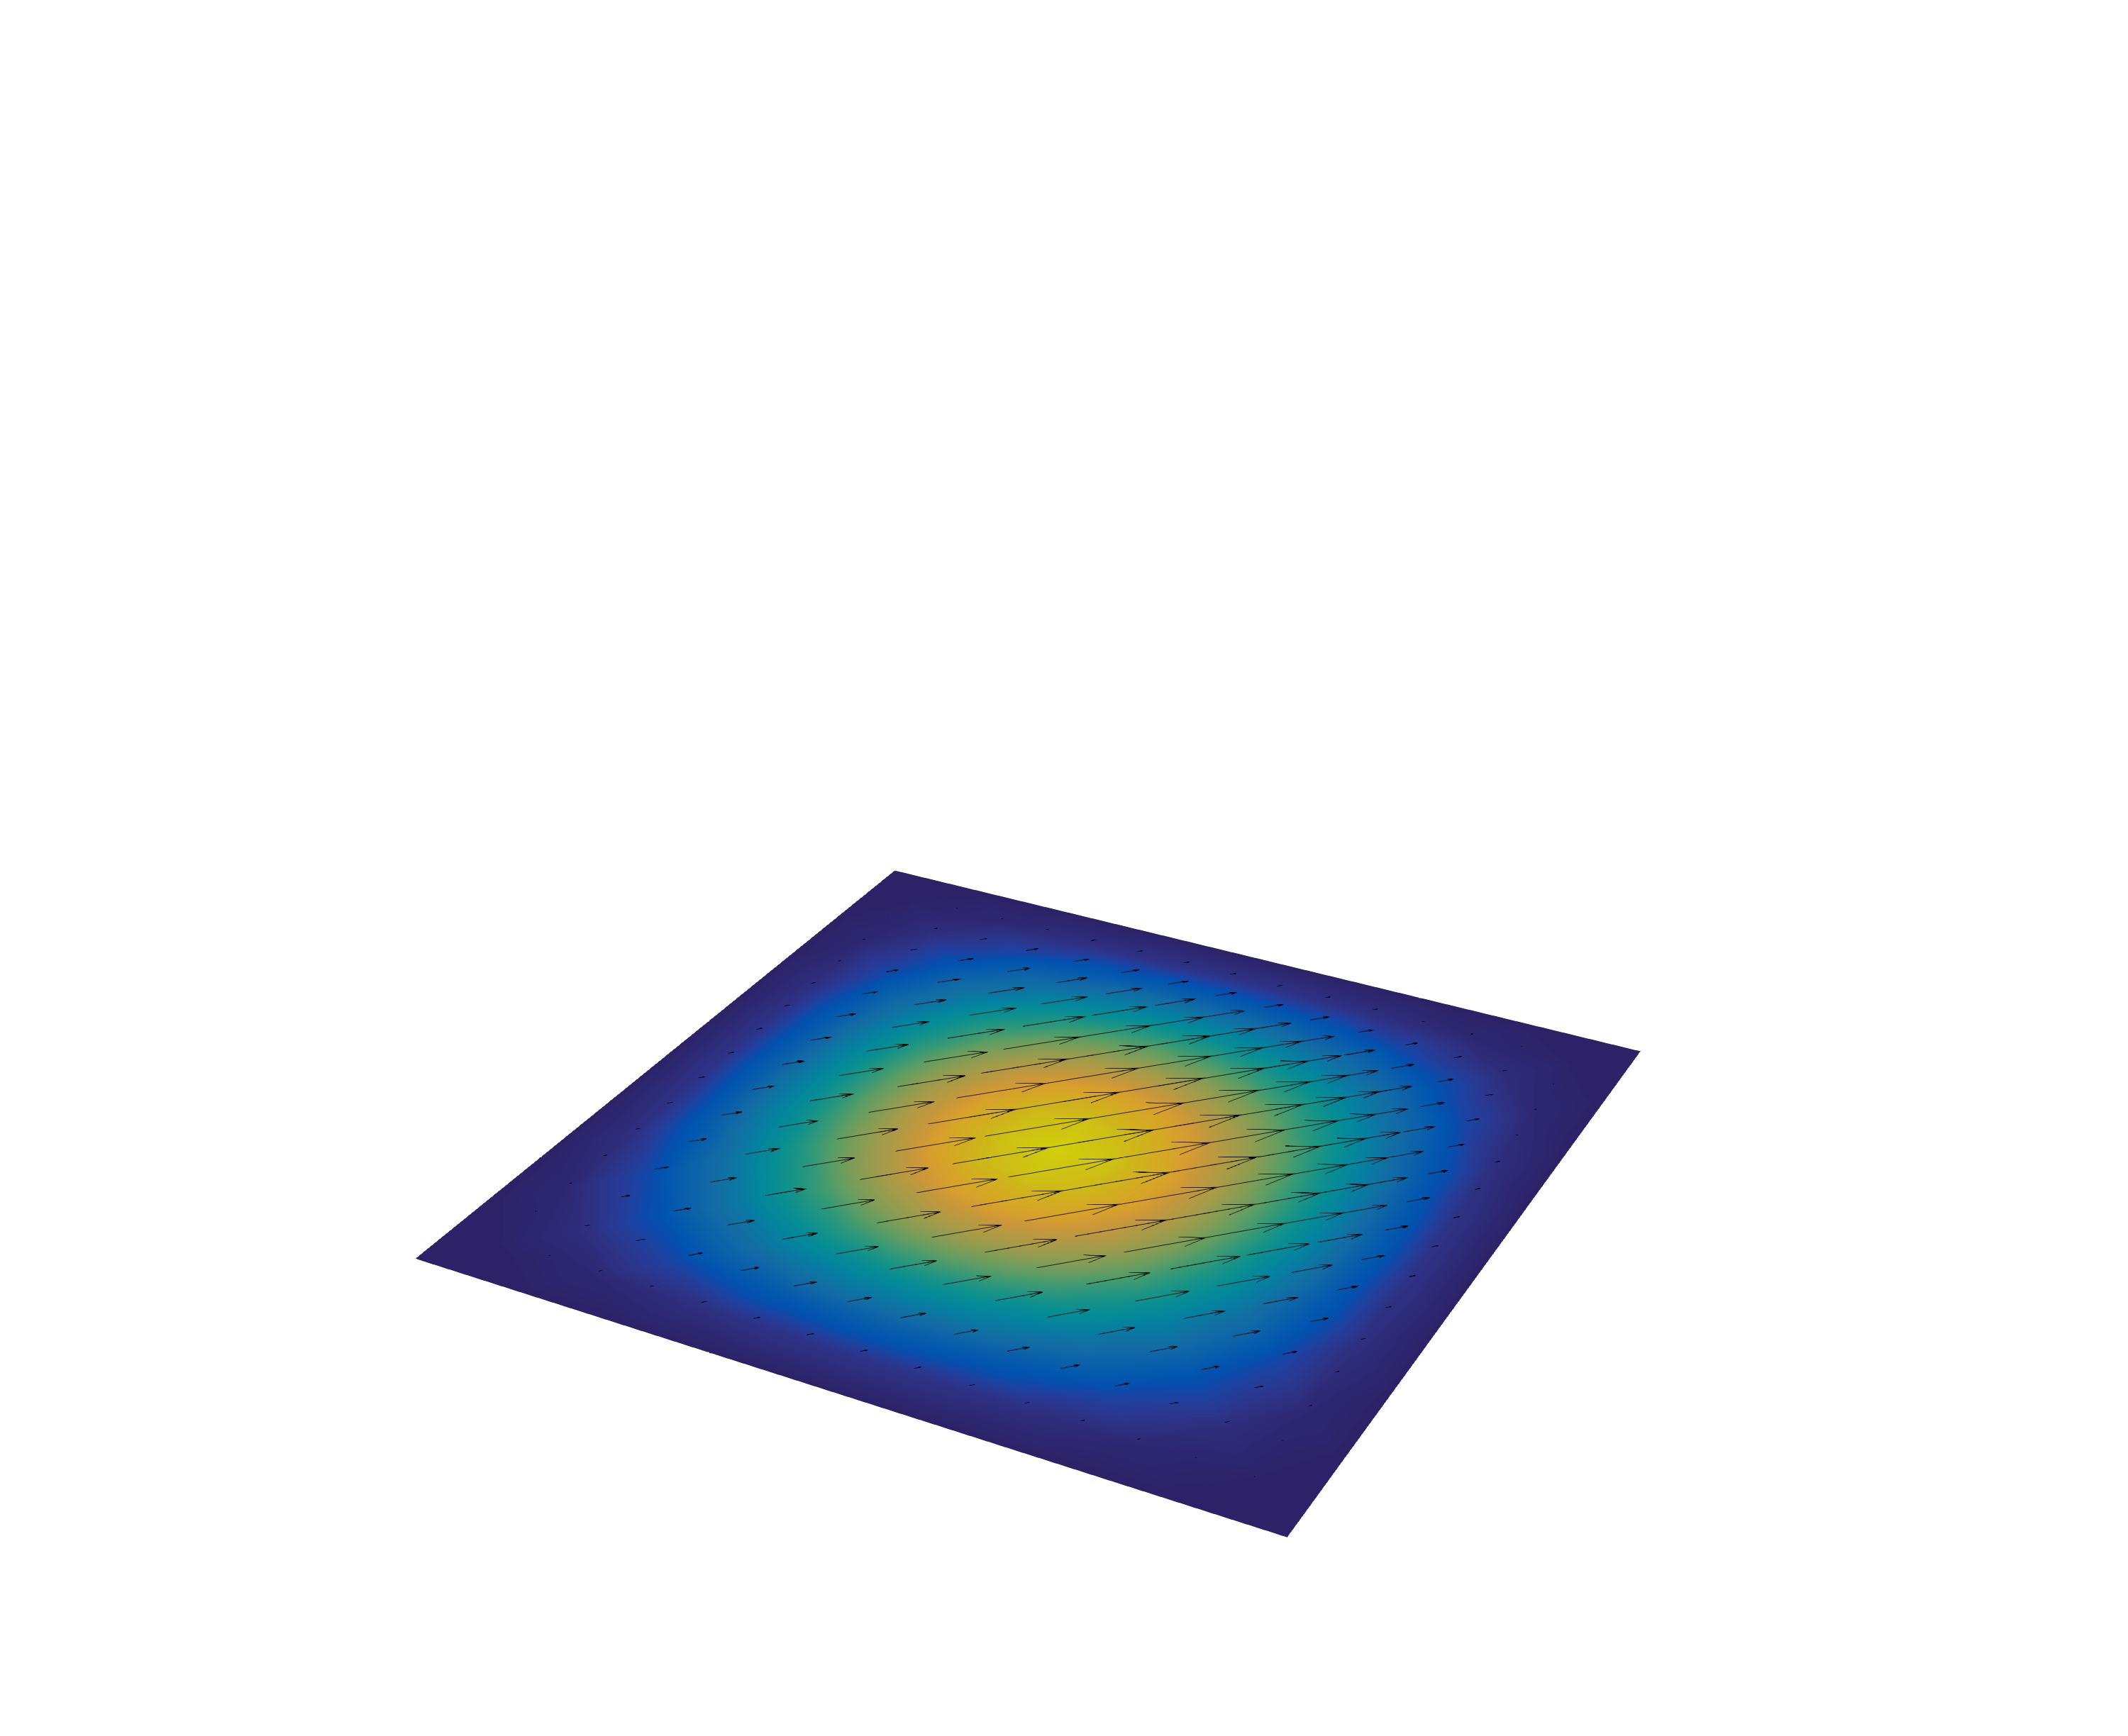
\includegraphics[width=\textwidth]{../media/fourier/fig-exact/print/slice-6.png}
      \caption{$x_3 = 2$}
    \end{subfigure}
    \begin{subfigure}[b]{0.49\textwidth}
      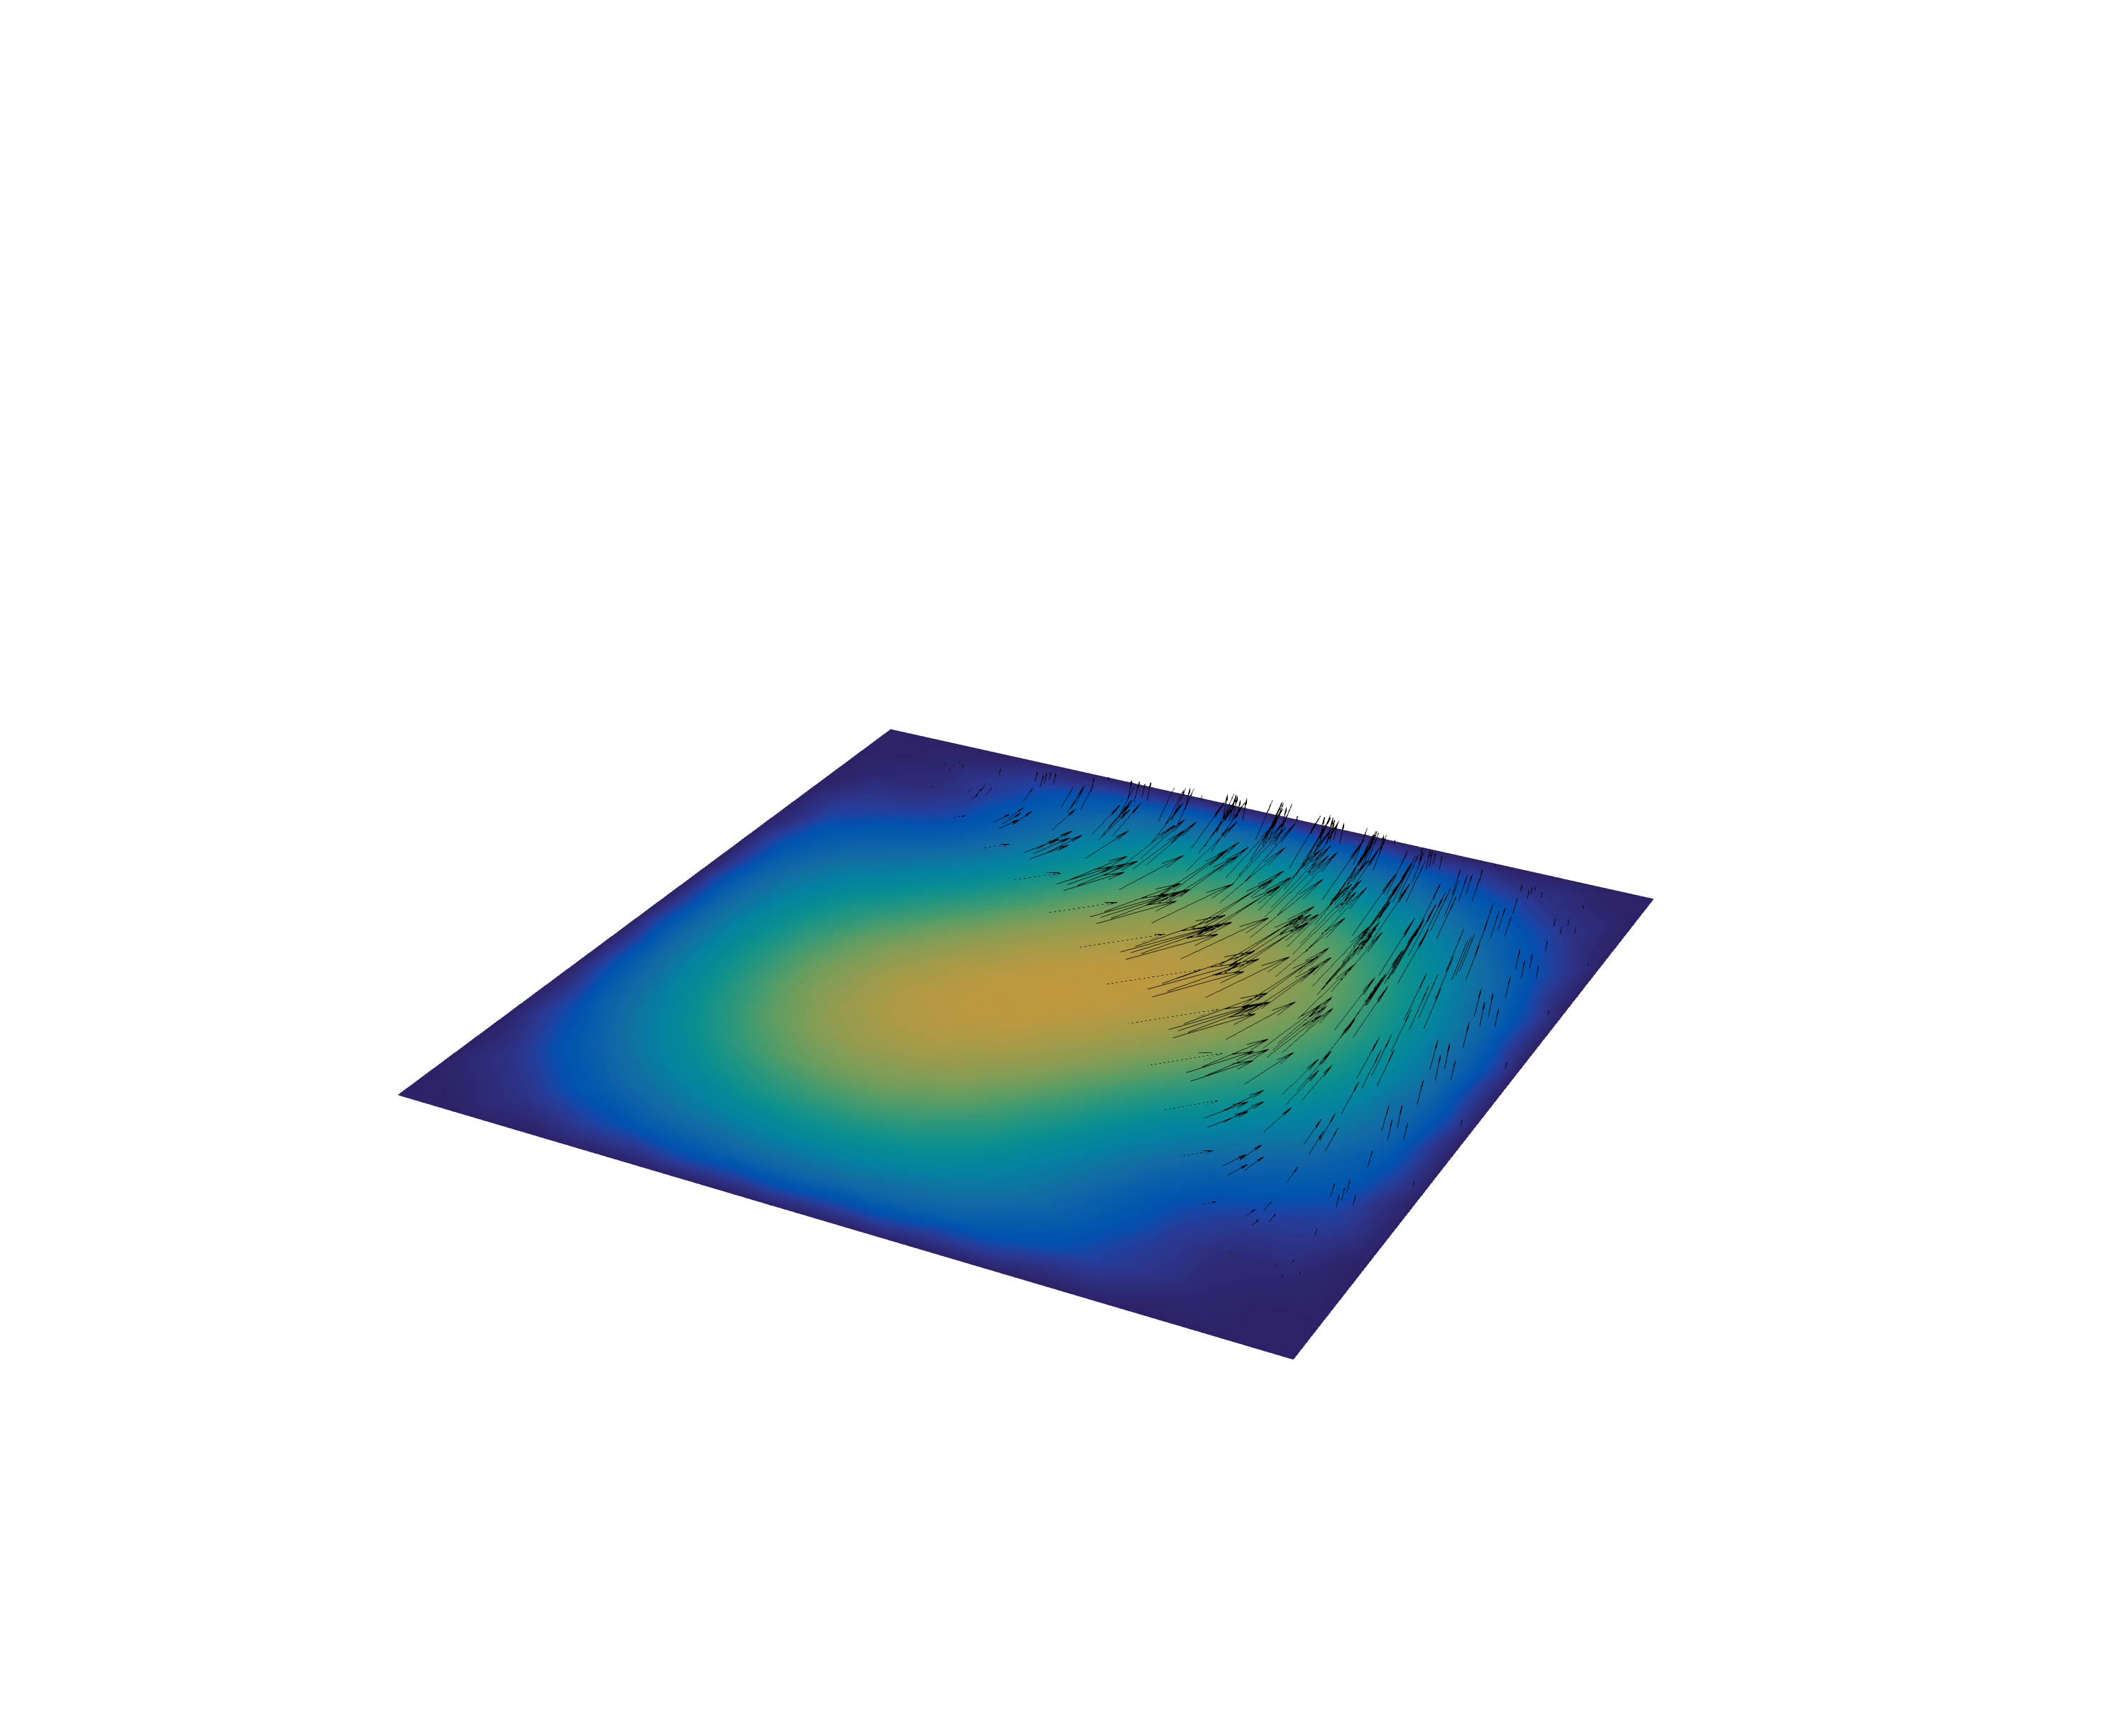
\includegraphics[width=\textwidth]{../media/fourier/fig-exact/print/slice-5.png}
      \caption{$x_3 = 1.6$}
    \end{subfigure}
    \begin{subfigure}[b]{0.49\textwidth}
      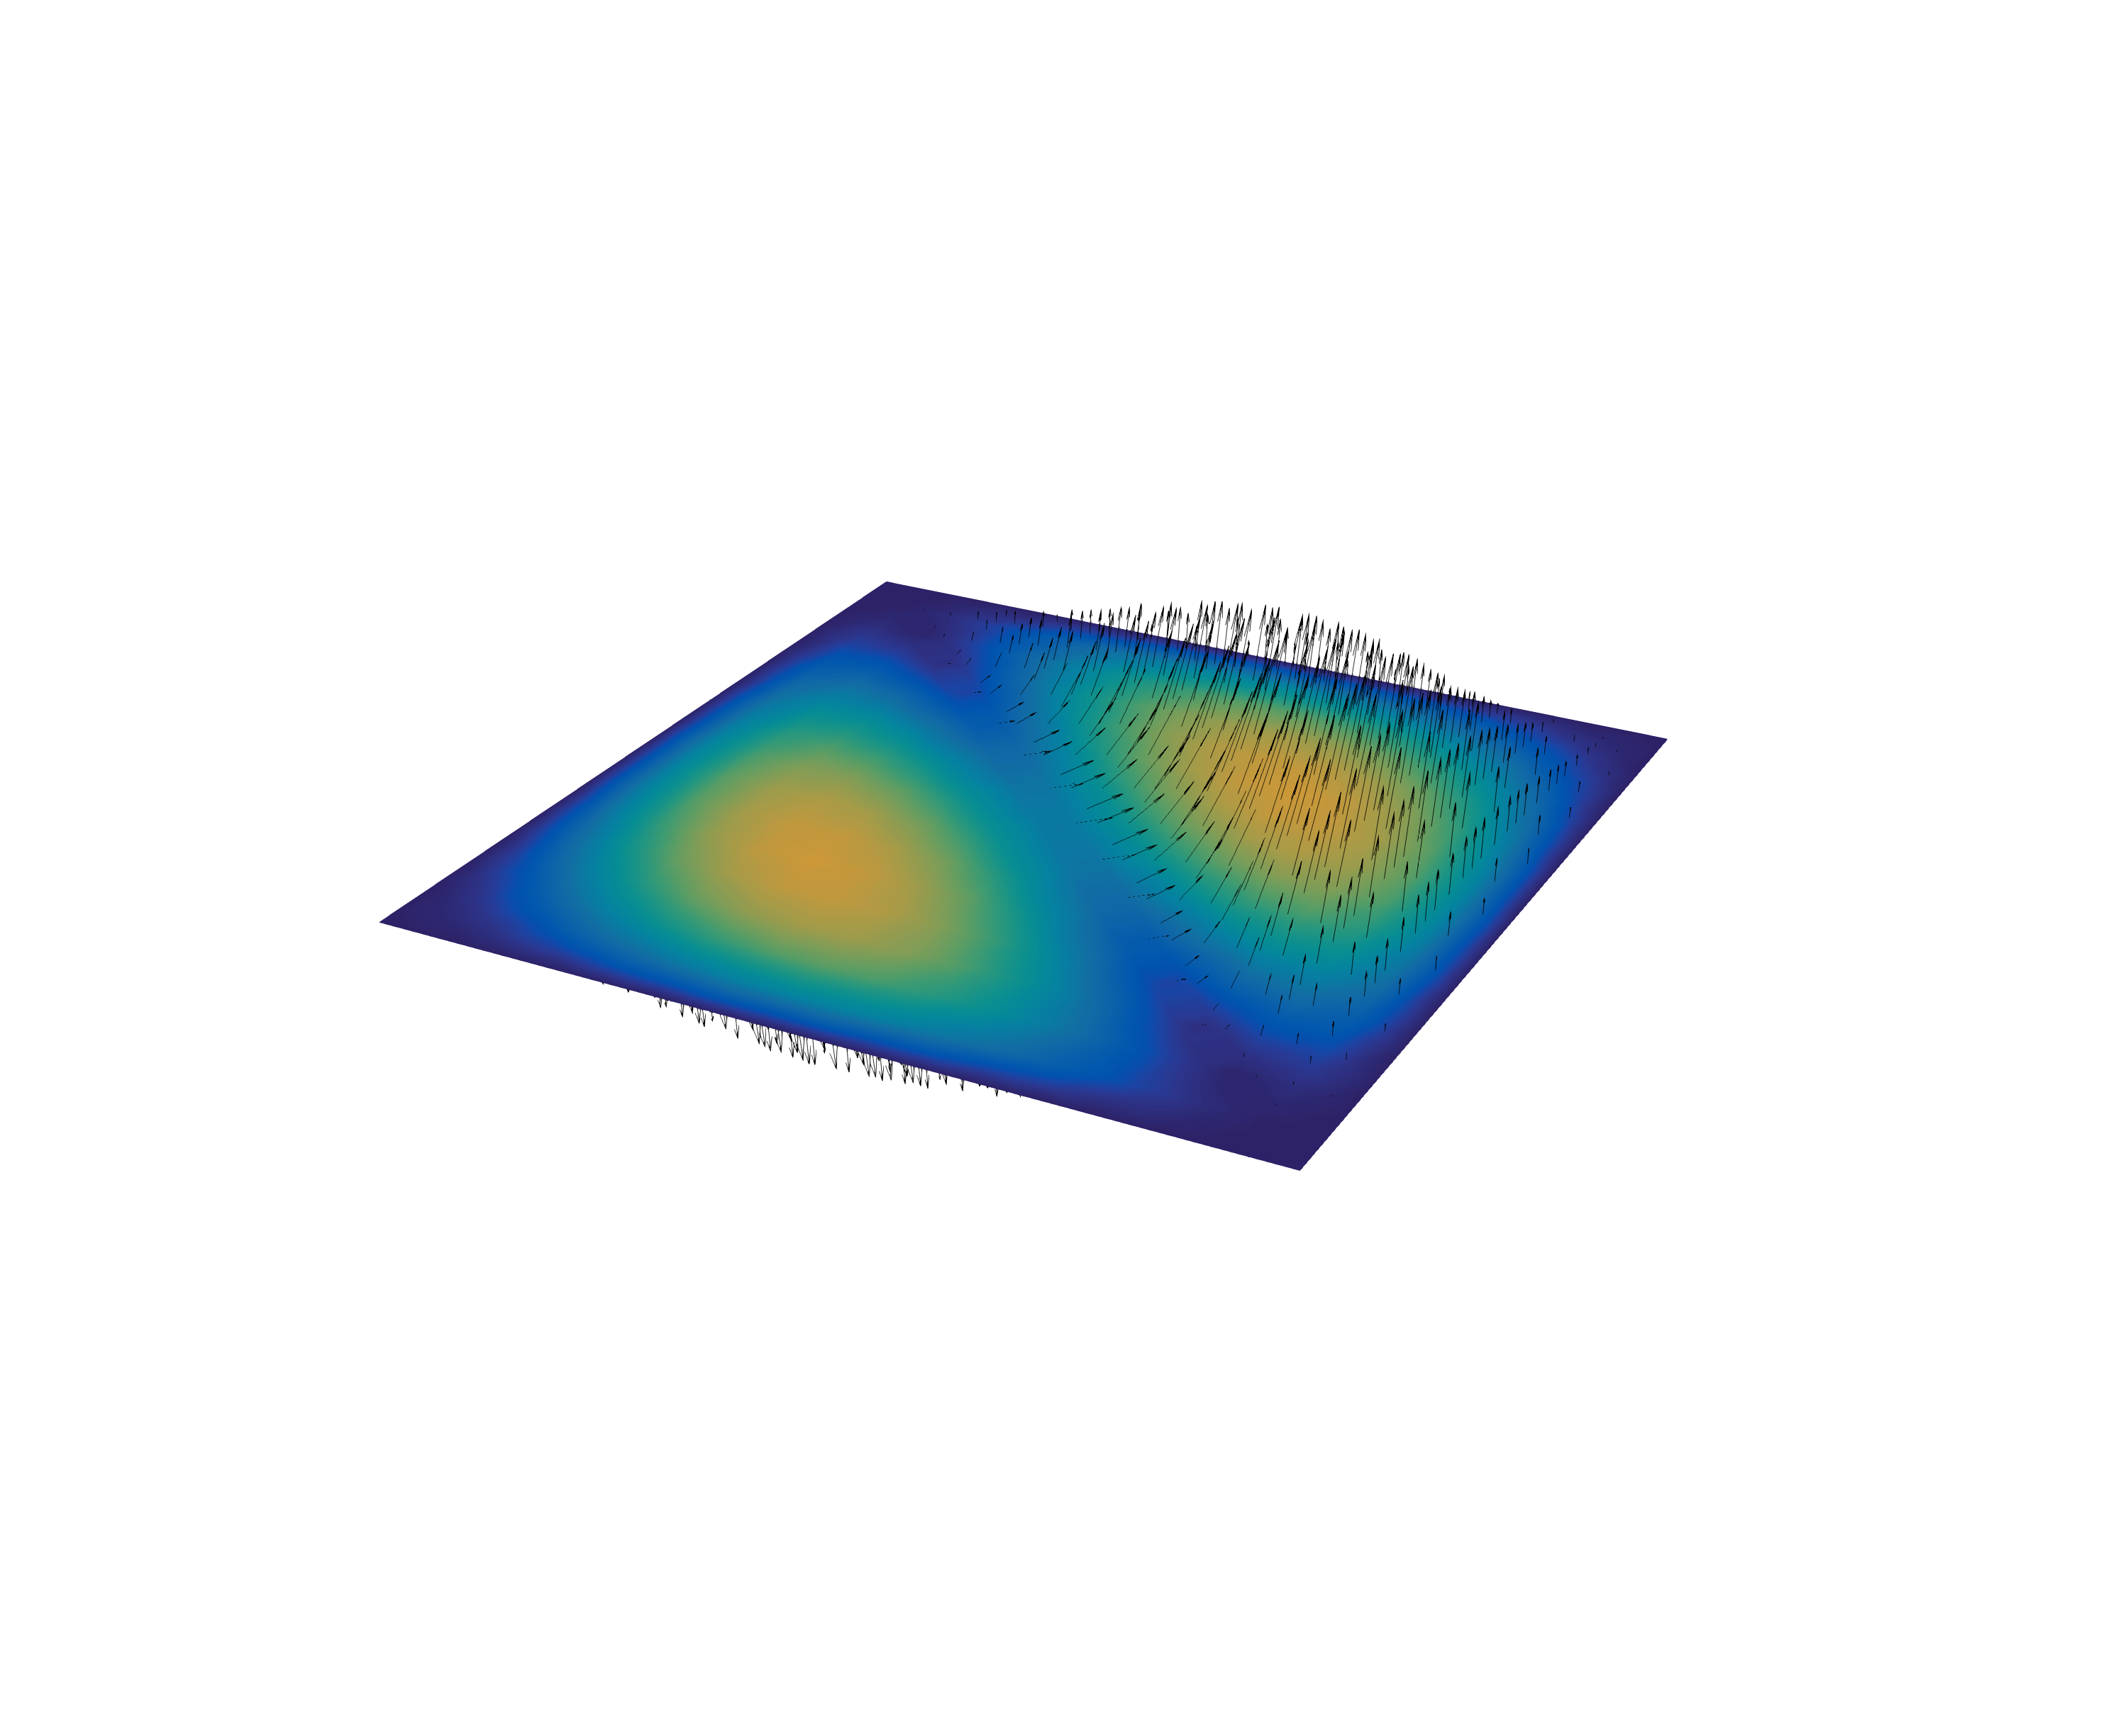
\includegraphics[width=\textwidth]{../media/fourier/fig-exact/print/slice-4.png}
      \caption{$x_3 = 1.2$}
    \end{subfigure}
    \begin{subfigure}[b]{0.49\textwidth}
      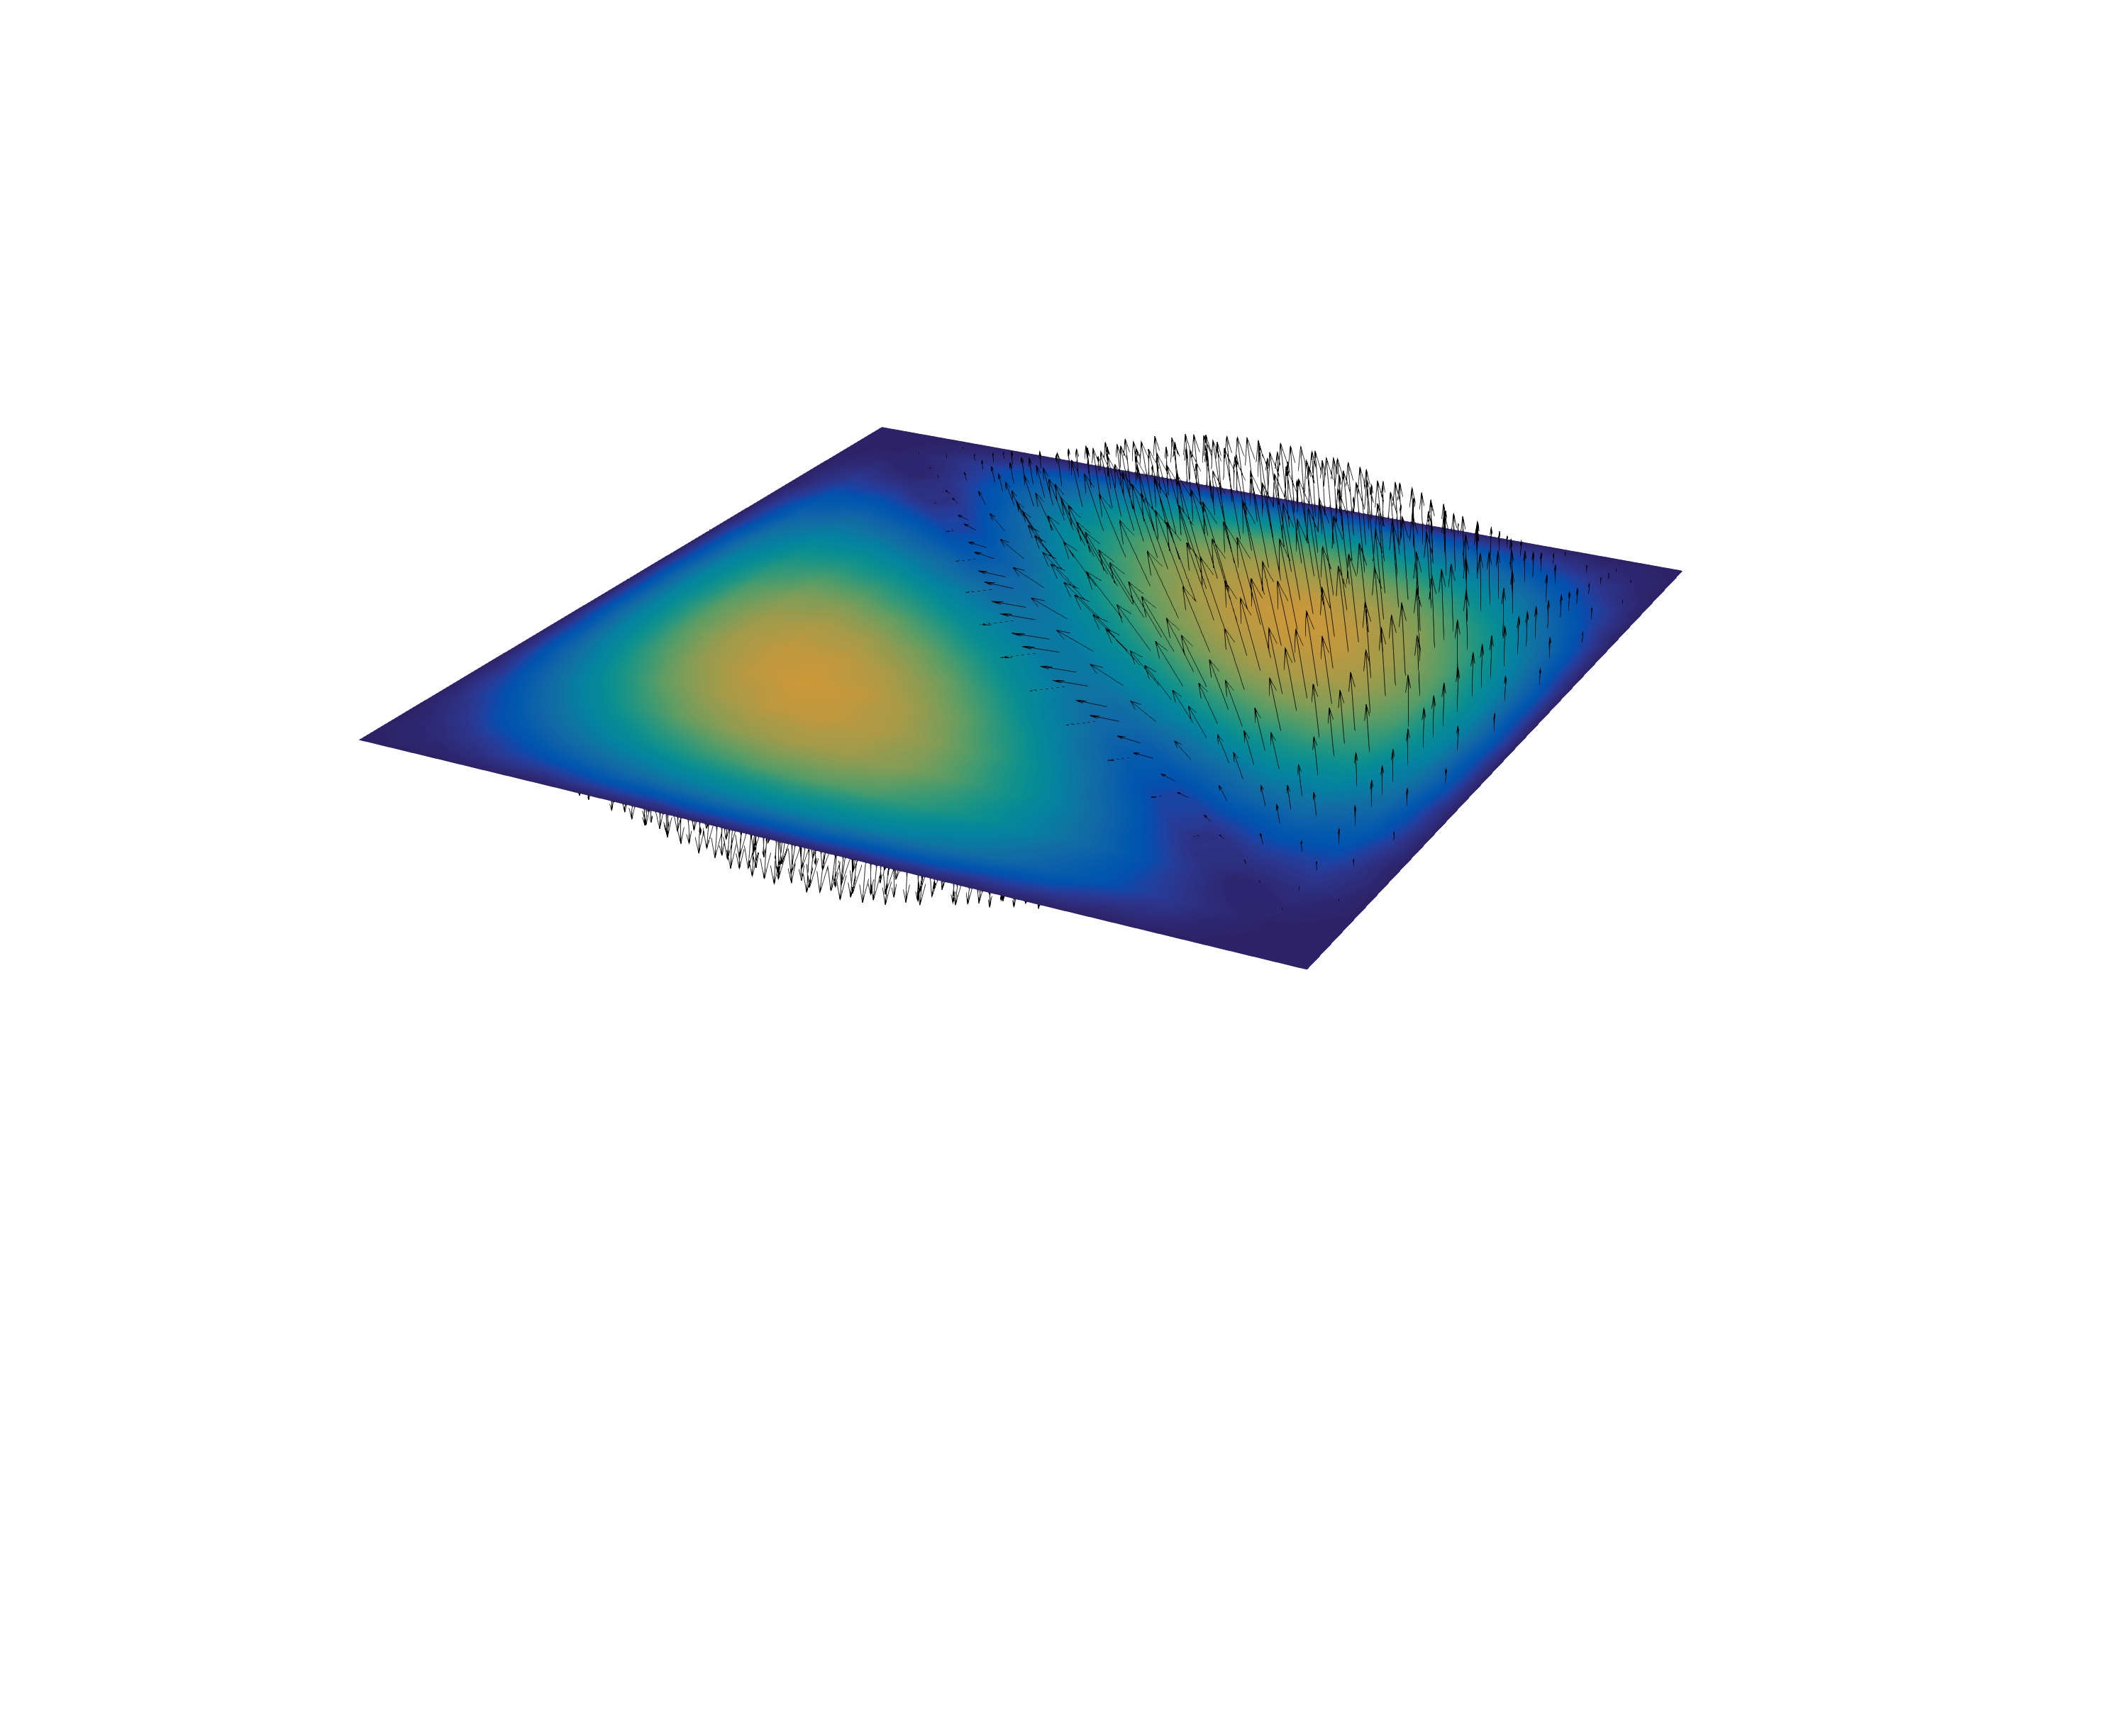
\includegraphics[width=\textwidth]{../media/fourier/fig-exact/print/slice-3.png}
      \caption{$x_3 = 0.8$}
    \end{subfigure}
    \begin{subfigure}[b]{0.49\textwidth}
      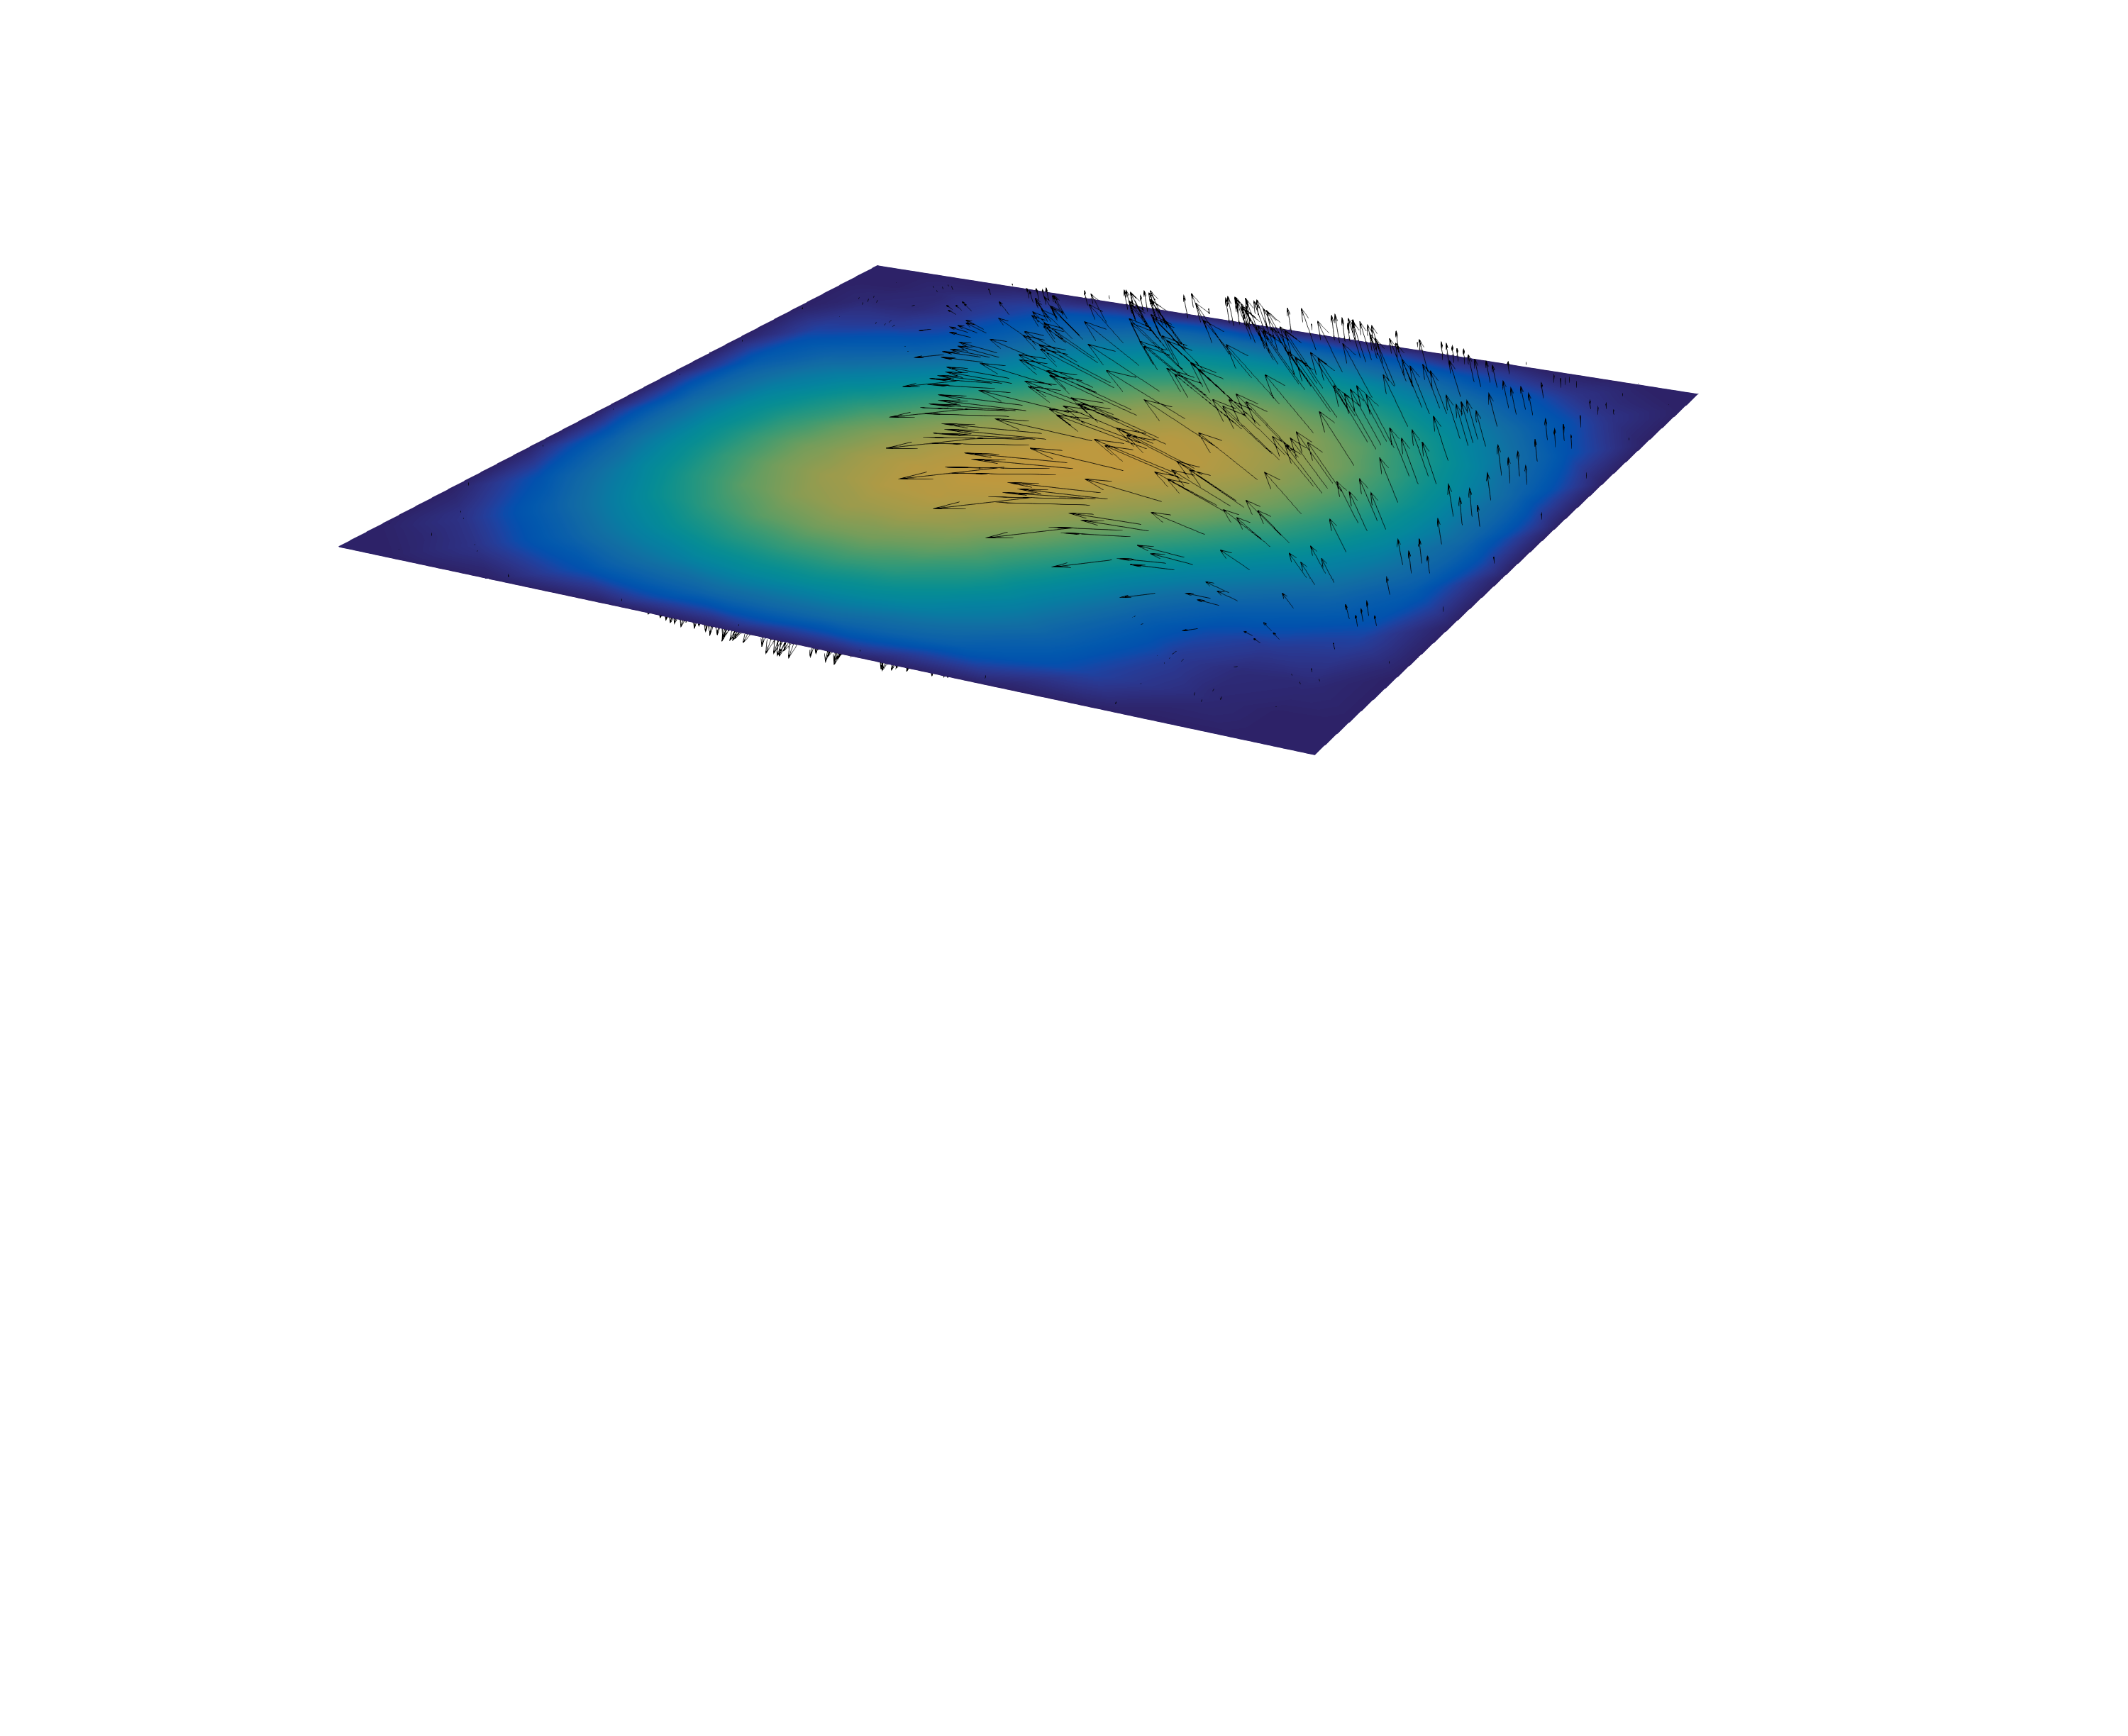
\includegraphics[width=\textwidth]{../media/fourier/fig-exact/print/slice-2.png}
      \caption{$x_3 = 0.4$}
    \end{subfigure}
    \begin{subfigure}[b]{0.49\textwidth}
      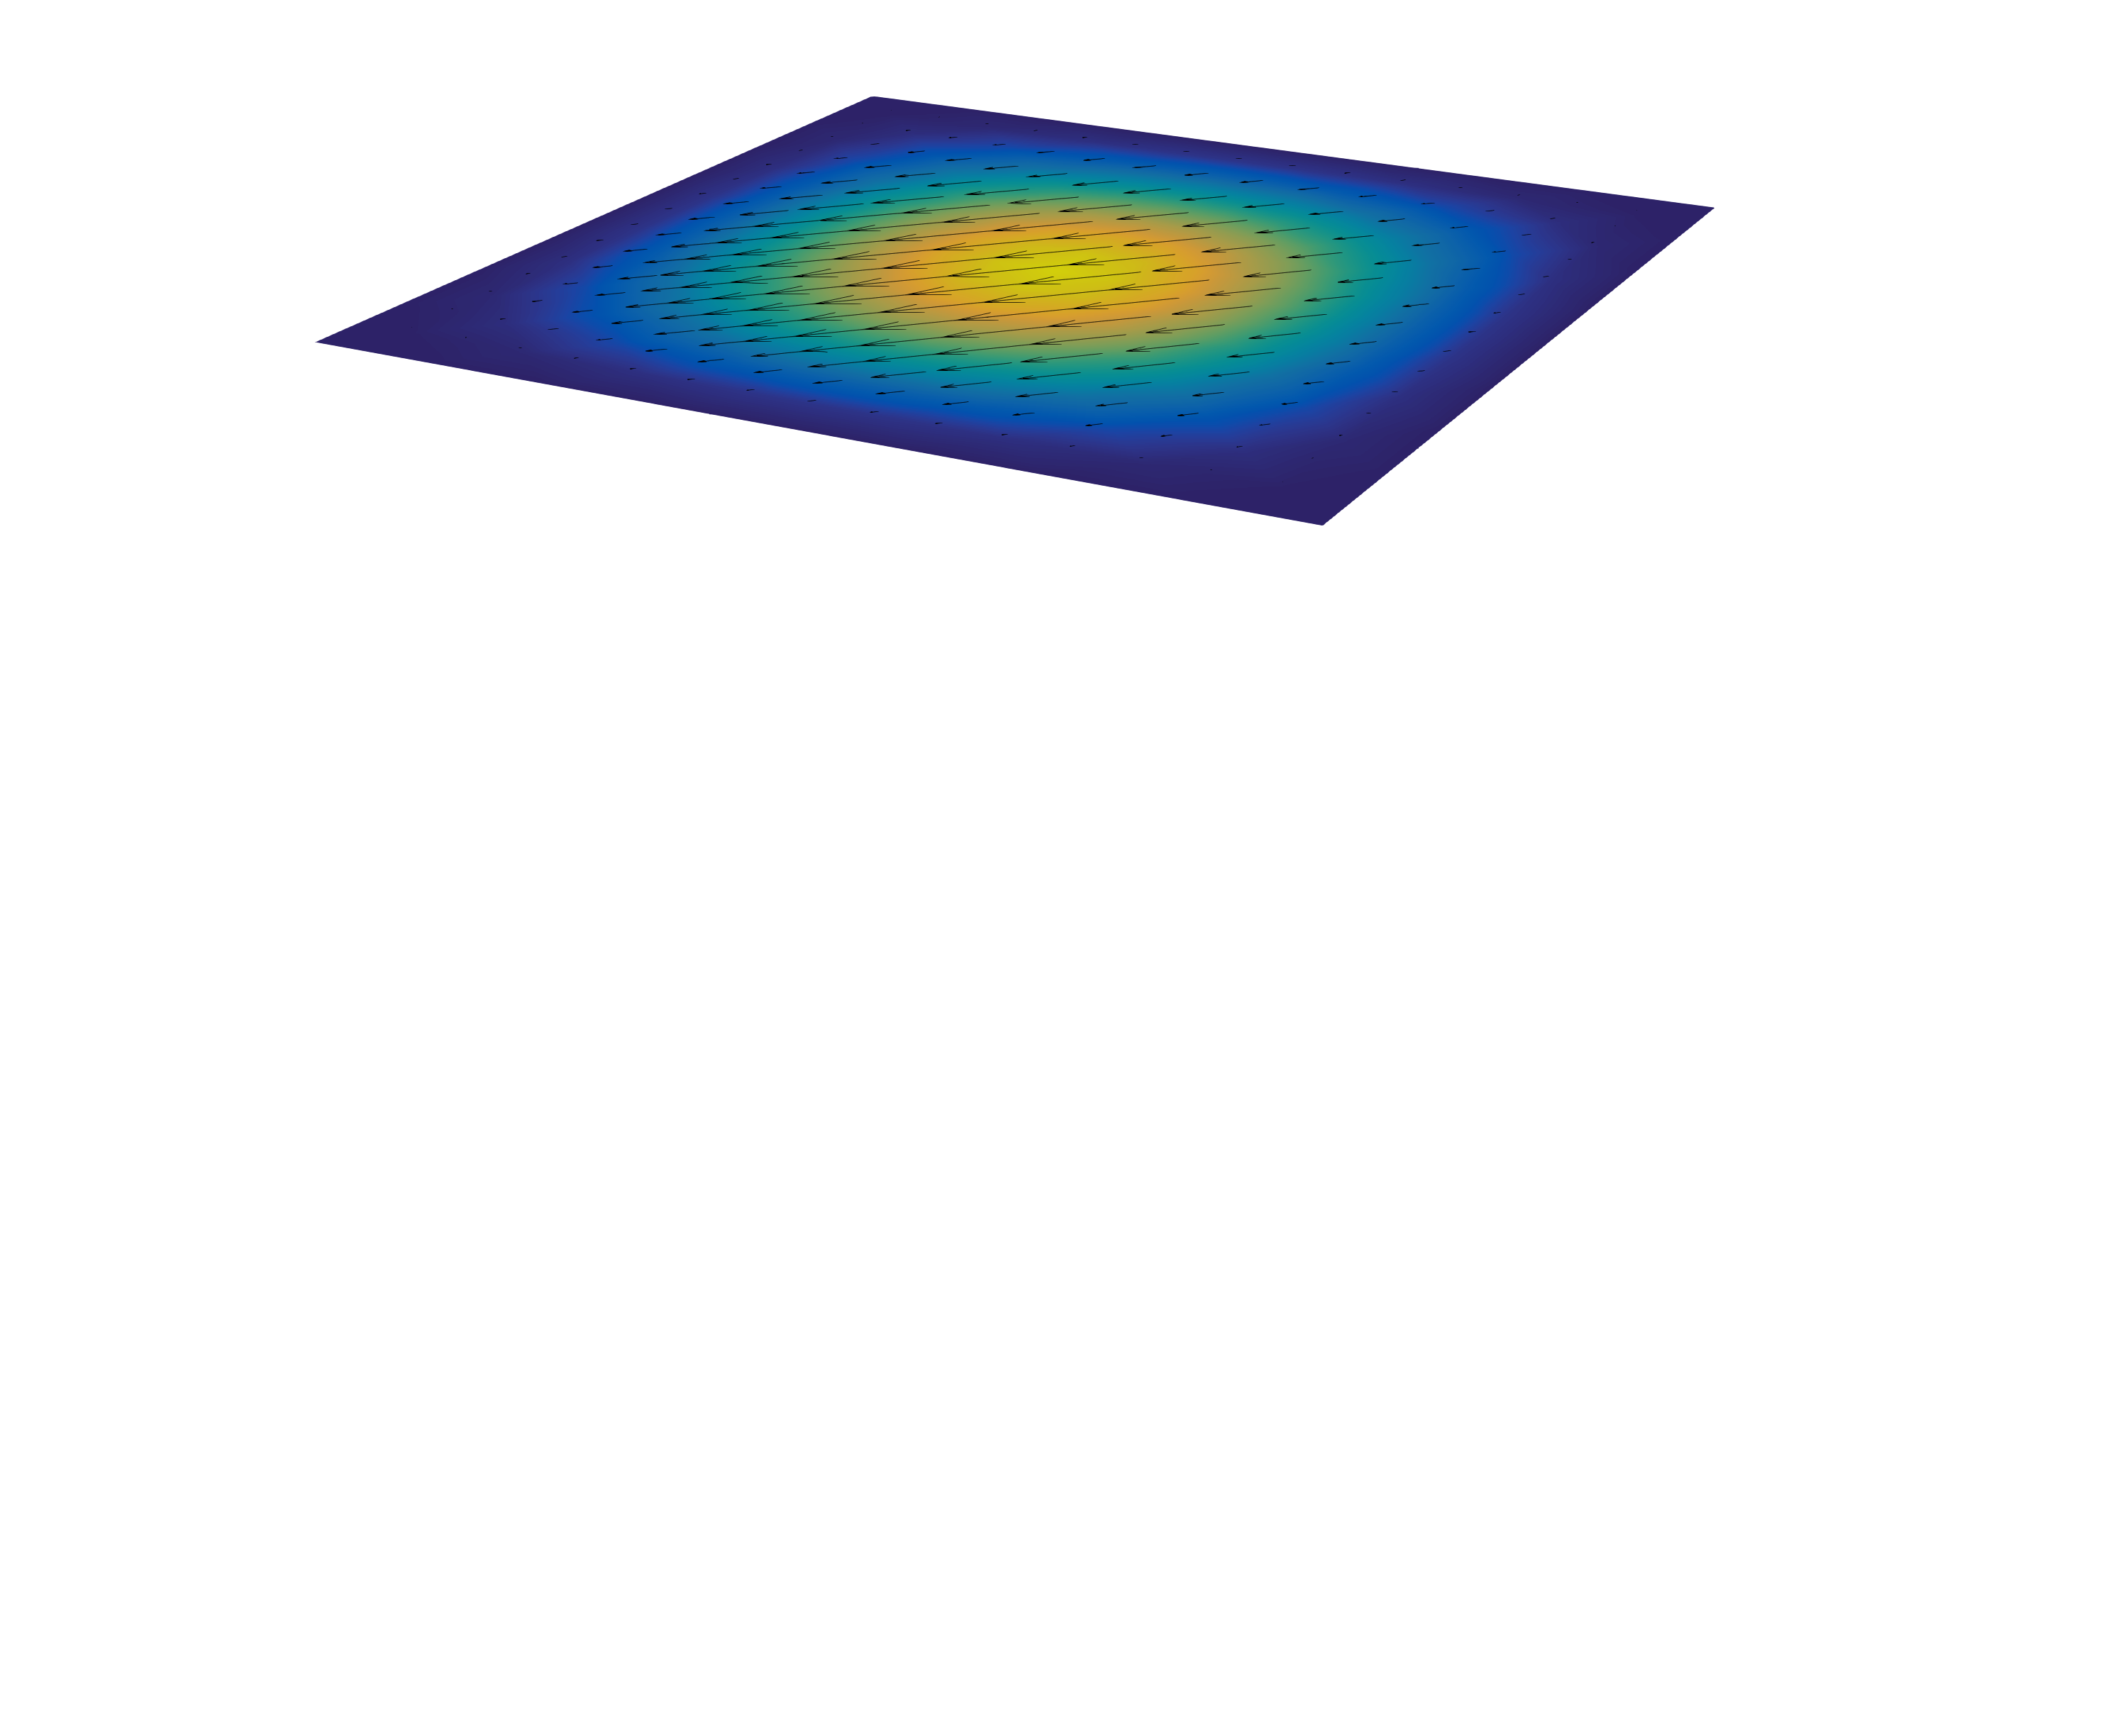
\includegraphics[width=\textwidth]{../media/fourier/fig-exact/print/slice-1.png}
      \caption{$x_3 = 0$}
    \end{subfigure}
    \caption{Représentation de la solution exacte
      (\ref{eq:stokes-exact-sol-1})-(\ref{eq:stokes-exact-sol-3}) du
      problème de Stokes (\ref{eq:stokes-u}), (\ref{eq:stokes-p}). La
      solution est représentée sur 6 plans horizontaux espacés
      régulièrement entre $x_3 = 0$ et $x_3 = 2$. L'échelle de couleur
      correspond à l'amplitude de $u$, tandis que les flèches indique
      la direction de $u$.}
    \label{fig:stokes-exact-sol}
  \end{center}
\end{figure}

\begin{figure}[t]
  \begin{center}
    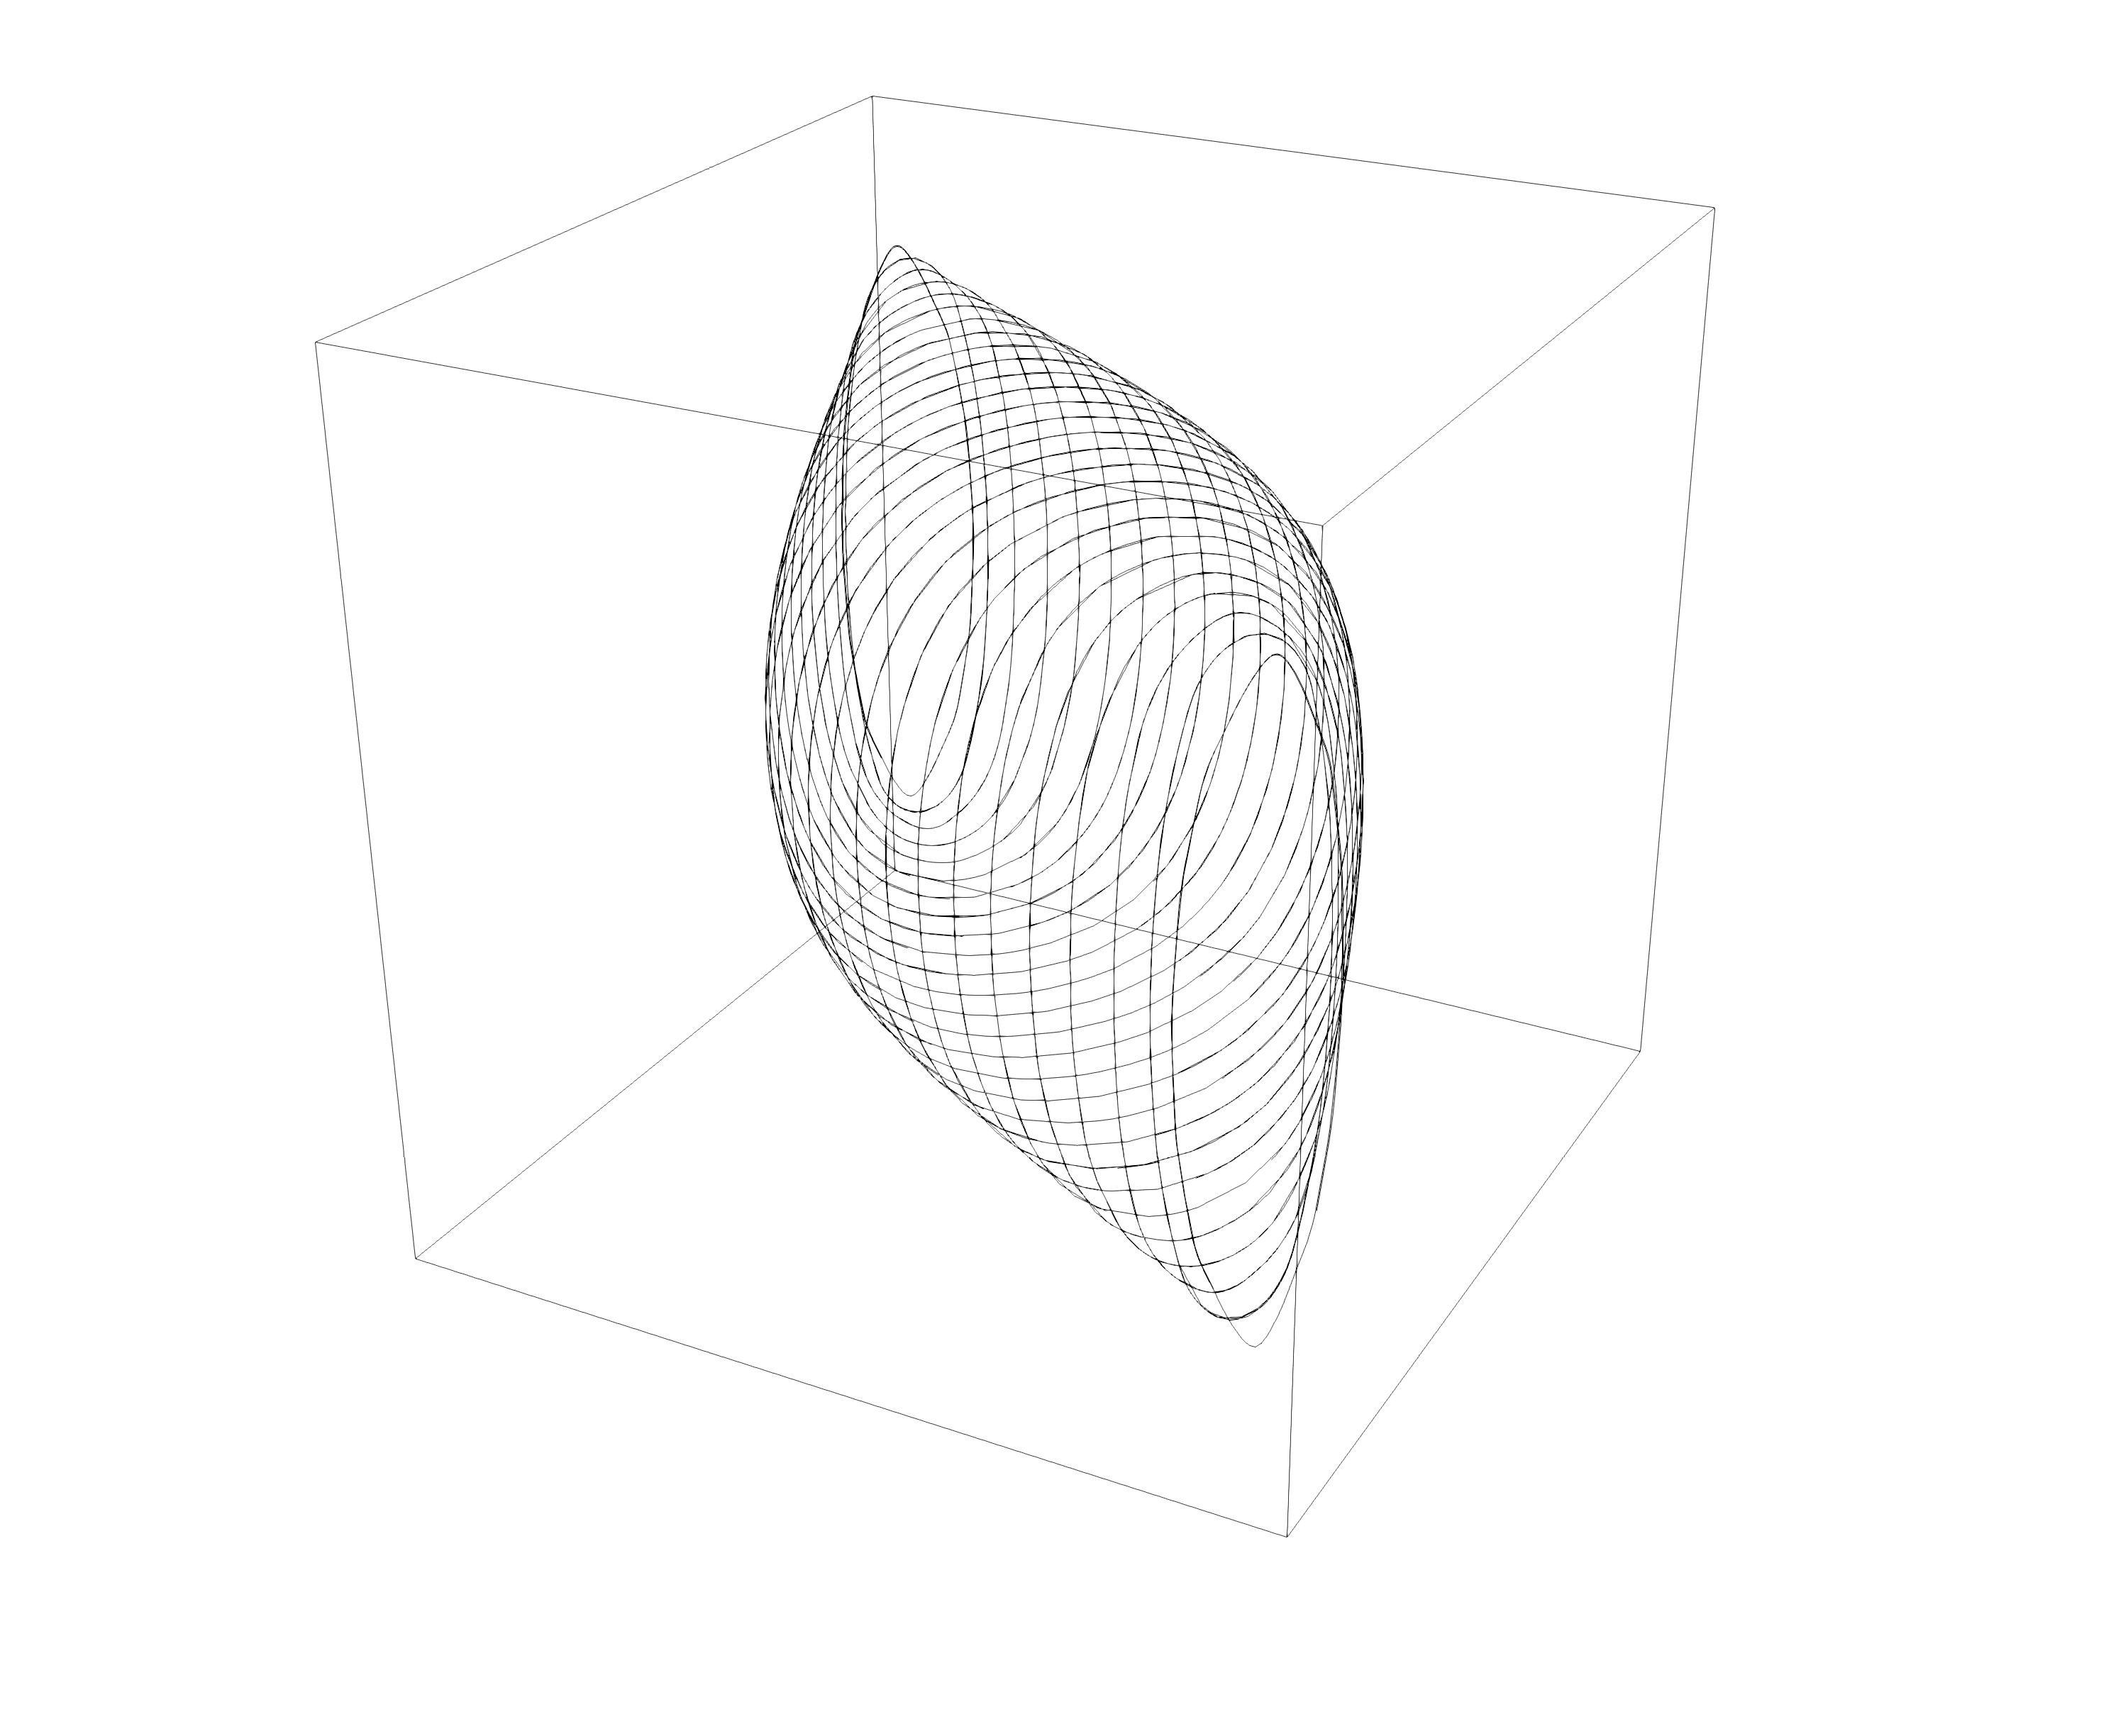
\includegraphics[width=\rasterimagewidth]{../media/fourier/fig-exact/print/streamlines.png}
    \caption{Lignes de courant de la vitesse $u$ définie par
      (\ref{eq:stokes-exact-sol-1})-(\ref{eq:stokes-exact-sol-2}) dans
      le domaine cubique $\Omega$, c'est-à-dire que $\thickness = 2$.}
    \label{fig:stokes-exact-sol-streamlines}
  \end{center}
\end{figure}


\subsection{Convergence de l'erreur}
On s'intéresse d'une part à la convergence de l'erreur d'approximation
de $u_{h,K}$ donnée par (\ref{eq:u-h-12}),(\ref{eq:u-h-3}) vers la
solution exacte
(\ref{eq:stokes-exact-sol-1})-(\ref{eq:stokes-exact-sol-2}), définie
par:
\begin{equation}
  e_{h,K}^{\mathrm{SF}} =
  \frac{\norm{u - u_{h,K}}_{L^2(\Omega)}}{\norm{u}_{L^2(\Omega)}},
\end{equation}
où le champ de vecteur $u$ est donné par
(\ref{eq:stokes-exact-sol-1})-(\ref{eq:stokes-exact-sol-2}).

On cherchera d'autre part à comparer $u_{h,K}$ (notée
$u_{h,K}^{\mathrm{SF}}$ dans la suite) avec la solution de
(\ref{eq:stokes-u}), (\ref{eq:stokes-p}) obtenue à l'aide d'une
méthode d'éléments finis $\mathbb P_1$bulle-$\mathbb P_1$ sur un
maillage tétraédrique classique (notée
$u_h^\mathrm{S3D}$ dans la suite). On note aussi l'erreur
\begin{equation}
  e_h^{\mathrm{S3D}} = \frac{\norm{u - u_h^{\mathrm{S3D}}}_{L^2(\Omega)}}{\norm{u}_{L^2(\Omega)}}.
\end{equation}

\subsubsection{Convergence de la somme partielle de Fourier}
On s'intéresse à la convergence de l'erreur $e_h^\mathrm{SF}$ en
fonction du nombre d'harmoniques $K$ dans la somme partielle de
$u_{h,K}$. On prend pour le maillage $\mathcal M_h$ du domaine $\Lambda$
une triangulation structurée de taille de maille $h = 2/64$. La
table \ref{tab:h-k-convergence} donne les valeurs de l'erreur
$e_{h,K}^\mathrm{SF}$ pour différents nombres d'harmoniques $K$ et
différentes épaisseurs $\thickness$ du domaine $\Omega$.

\begin{table}[t]
  \caption{Erreur $e_{h,K}^\mathrm{SF}$ entre la solution exacte et la
    série de Fourier tronquée à l'ordre $K$.}
  \label{tab:h-k-convergence}
  \begin{center}
    \begin{tabular}{@{}rrrrrr@{}}
      \toprule
                   %& $K = 1$ & $K = 2$ & $K = 3$ & $K = 4$ & $K = 5$ & $K = 6$ & $K = 7$ & $K = 8$\\
      $\epsilon$   & $K = 1$ & $K = 3$ & $K = 5$ & $K = 7$ & $K = 9$\\
      \cmidrule{1-6}
      $2$      & \num{0.8918E-02} & \num{0.1216E-02} & \num{0.5207E-03} & \num{0.4378E-03} & \num{0.4259E-03} \\
      $0.2$    & \num{0.1238E-01} & \num{0.1654E-02} & \num{0.4547E-03} & \num{0.1882E-03} & \num{0.1117E-03} \\
      $0.02$   & \num{0.1245E-01} & \num{0.1662E-02} & \num{0.4508E-03} & \num{0.1727E-03} & \num{0.8142E-04} \\
      %
      %$h = 2$      & \num{0.89186348E-02} & \num{0.89189885E-02} & \num{0.12167724E-02} & \num{0.12172997E-02} & \num{0.52070528E-03} & \num{0.52114649E-03} & \num{0.43781666E-03} & \num{0.43807398E-03} & \num{0.42595367E-03} \\
      %$h = 0.2$    & \num{0.12389603E-01} & \num{0.12389604E-01} & \num{0.16543681E-02} & \num{0.16543708E-02} & \num{0.45478885E-03} & \num{0.45479262E-03} & \num{0.18823592E-03} & \num{0.18823987E-03} & \num{0.11171968E-03} \\
      %$h = 0.02$   & \num{0.12455460E-01} & \num{0.12455460E-01} & \num{0.16621111E-02} & \num{0.16621111E-02} & \num{0.45086937E-03} & \num{0.45086937E-03} & \num{0.17279275E-03} & \num{0.17279275E-03} & \num{0.81428389E-04} \\
      \bottomrule
    \end{tabular}
  \end{center}
\end{table}


\subsubsection{Convergence en fonction du maillage}
On s'intéresse à la convergence de l'erreur $e_{h,K}^\mathrm{SF}$ en
fonction de la taille de maille $h$ de la subdivision $\mathcal M_h$ du domaine
$\Lambda$. Le tableau \ref{tab:n-h-convergence} donne les valeurs de
l'erreur pour différentes tailles de maille $h$ et différentes
épaisseurs $\thickness$ du domaine $\Omega$.

\begin{table}[t]
  \caption{Erreur $e_{h,K}^\mathrm{SF}$ en fonction de $h$ et de
    la taille de maille $h$ et de l'épaisseur $\thickness$ lorsque $K
    = 20$.}
  \label{tab:n-h-convergence}
  \begin{center}
    \begin{tabular}{@{}rrrrrr@{}}
      \toprule
      $\epsilon$ & $h = 0.25$ & $h = 0.125$ & $h = 0.0625$ & $h = 0.03125$ & $h = 0.015625$ \\
      \cmidrule{1-6}
      $2$      & \num{0.9765E-01} & \num{0.2611E-01} & \num{0.6698E-02} & \num{0.1688E-02} & \num{0.4232E-03} \\
      $0.2$    & \num{0.4184E-02} & \num{0.2342E-02} & \num{0.9966E-03} & \num{0.2962E-03} & \num{0.7794E-04} \\
      $0.02$   & \num{0.3977E-04} & \num{0.1166E-04} & \num{0.9187E-05} & \num{0.1121E-04} & \num{0.1210E-04} \\
      %$h = 2$      & \num{0.97650317E-01} & \num{0.26117175E-01} & \num{0.66981324E-02} & \num{0.16888002E-02} & \num{0.42326195E-03} \\
      %$h = 0.2$    & \num{0.41848104E-02} & \num{0.23426567E-02} & \num{0.99662780E-03} & \num{0.29620176E-03} & \num{0.77949986E-04} \\
      %$h = 0.02$   & \num{0.39774924E-04} & \num{0.11660001E-04} & \num{0.91876790E-05} & \num{0.11211307E-04} & \num{0.12101410E-04} \\
      \bottomrule
    \end{tabular}
  \end{center}
\end{table}


\subsubsection{Comparaison des erreur $e_h^{\mathrm{SF}}$ et
  $e_h^{\mathrm{S3D}}$} On s'intéresse maintenant à comparer la
précision des calculs $u_{h,K}^\mathrm{SF}$ et
$u_h^{\mathrm{S3D}}$. Ici on a choisi $K = 20$ et $h = 2/64$. La table
\ref{tab:e-sf-e-s3d-convergence} donne la valeur des erreurs pour
différents épaisseurs $\thickness$ du domaine $\Omega$. La figure
\ref{fig:e-sf-e-s3d-convergence} représente les même données sous
forme graphique.

\begin{table}[t]
  \caption{Erreurs $e_{h,K}^\mathrm{SF}$ et $e_h^\mathrm{S3D}$ en fonction
    de l'épaisseur $\thickness$ lorsque $K = 20$ et $h = 2/64$.}
  \label{tab:e-sf-e-s3d-convergence}
  \begin{center}
    \begin{tabular}{@{}rrrrrrrrrrr@{}}
      \toprule
      & $\thickness = 0.020$
      %& $\thickness = 0.033$
      & $\thickness = 0.055$
      %& $\thickness = 0.092$
      & $\thickness = 0.154$
      %& $\thickness = 0.258$
      & $\thickness = 0.430$
      %& $\thickness = 0.718$
      & $\thickness = 1.198$ \\
      %& $\thickness = 2$ \\
      \cmidrule{2-6}
      $e_{h,K}^\mathrm{SF}$  & \num{0.1121E-04} & \num{0.8356E-04} & \num{0.2478E-03} & \num{0.4944E-03} & \num{0.1225E-02}\\
      $e_h^\mathrm{S3D}$ & \num{0.1426E-02} & \num{0.1351E-02} & \num{0.1175E-02} & \num{0.9317E-03} & \num{0.6221E-03}\\
      %$e_h^\mathrm{SF}$  & \num{0.11211307E-04} & \num{0.30500446E-04} & \num{0.83562271E-04} & \num{0.16100704E-03} & \num{0.24780044E-03} & \num{0.34930482E-03} & \num{0.49448033E-03} & \num{0.76153942E-03} & \num{0.12254762E-02} & \num{0.16888002E-02} \\
      %$e_h^\mathrm{S3D}$ & \num{0.14265133E-02} & \num{0.14010261E-02} & \num{0.13516086E-02} & \num{0.12761443E-02} & \num{0.11759665E-02} & \num{0.10615871E-02} & \num{0.93173182E-03} & \num{0.78897224E-03} & \num{0.62210445E-03} & \num{0.84532577E-03} \\
      \bottomrule
    \end{tabular}
  \end{center}
\end{table}

\begin{figure}
  \begin{center}
    \input{../media/fourier/convergence/sf-convergence.tex}
    \caption{Erreurs $e_{h,K}^\mathrm{SF}$ et $e_h^\mathrm{S3D}$ en fonction
    de l'épaisseur $\thickness$ lorsque $K = 20$ et $h = 2/64$.}
    \label{fig:e-sf-e-s3d-convergence}
  \end{center}
\end{figure}

Finalement, on compare les temps CPU pour chaque schéma, ainsi
que le nombre d'itérations de l'algorithme GMRES pour résoudre le
système linéaire dans le cas du schéma S3D, dont les résultats sont
synthétisés par la table \ref{tab:e-sf-e-s3d-cpu-cost}. Ici on a
compare les performances entre le temps de calculs du modèle F3D et SF
en variant l'épaisseur $\thickness$ du domaine entre \num{2e-2} et \num{1.19}.

\begin{table}[t]
  \caption{Comparaison des performances entre les schémas permettant
    de calculer $u_{h,K}^{\mathrm{SF}}$ et $u_h^\mathrm{S3D}$ en
    fonction de l'épaisseur $\thickness$. Les calculs
    sont effectués sur un machine équipée d'un processeur Intel$^{\tiny{\textregistered}}$ Xeon$^{\tiny{\textregistered}}$
    E5-2620 v2 @ 2.1\si{\giga\hertz} et 32Go de RAM.}
  \label{tab:e-sf-e-s3d-cpu-cost}
  \begin{center}
    \begin{tabular}{@{}lrrrrr@{}}
      \toprule
      & $\thickness = 0.020$
      %& $\thickness = 0.033$
      & $\thickness = 0.055$
      %& $\thickness = 0.092$
      & $\thickness = 0.154$
      %& $\thickness = 0.258$
      & $\thickness = 0.430$
      %& $\thickness = 0.718$
      & $\thickness = 1.198$ \\
      %& $\thickness = 2$ \\
      \cmidrule{2-6}
      F3D  \\
      \hphantom{a} $T_\text{CPU}$ [\si{\second}] & 4587 & 2694 & 1343 & 753 & 753 \\
      \hphantom{a} itérations GMRES           & 901 & 609  & 327  & 184 & 133 \\
      SF \\
      \hphantom{a} $T_\text{CPU}$ [\si{\second}] & 43 & 45   & 43   & 44  & 45  \\
      \bottomrule
    \end{tabular}
  \end{center}
\end{table}
